\pagebreak

\section{An Interaction Model for De-identification of Human Data held by External Custodians} \label{sec:Simmons2018}

The previous sections of this chapter explained that data de-identification, particularly of spatio-temporal datasets such as the \afl{} dataset used in this thesis, is non-trivial to perform correctly. The analysis of trade-offs in \secref{sec:trade-off} revealed that common methods such as removing dates and venues, offsetting times, and substituting player names with random codes fail to prevent re-identification. Use of a point cloud data structure to represent team formations at each time instant was identified as the most theoretically promising in terms of individual privacy protection without destroying the ability to analyse the team as a whole. However, this method is rarely used in practice, and requires writing custom software to implement.

The challenge is that for all data to be \textit{non-identifiable}, the de-identification must be performed by the data custodian, i.e. the football club, who do not have the technical resources to apply sophisticated de-identification approaches. Thus despite the theoretical benefits of the approach identified by the previous sections, it could not be realised in practice under the common interaction model where the full burden of carrying out the data de-identification process is placed upon the data custodian without any involvement from the researchers that plan to analyse the data.

To ensure that secure de-identification approaches can be applied in practice, it was necessary to reconsider the interaction between data custodians and researchers. The goal was to find a solution whereby researchers could be involved in specifying the most appropriate de-identification process while still ensuring that the data custodian remained in control of the underlying identifiable data. The solution was formalised in terms of an interaction model and implemented as a de-identification portal. The portal was used to request the \afl{} datasets used in thesis and to automatically de-identify the data as they passed through the portal using the point cloud method identified in the previous section.

\textit{This section of the thesis was published as \fullcite{Simmons2018}. An authorship statement for the paper can be found in \appendixref{appendix:authorship}.}

\subsection{Abstract}

Reuse of pre-existing industry datasets for research purposes requires a
multi-stakeholder solution that balances the researcher's analysis
objectives with the need to engage the industry data custodian, whilst
respecting the privacy rights of human data subjects. Current methods
place the burden on the data custodian, whom may not be sufficiently
trained to fully appreciate the nuances of data de-identification.
Modelling of functional, quality, and emotional goals is used to arrive at a
de-identification in the cloud approach whereby the researcher
proposes analyses along with the extraction and de-identification
operations, while engaging the industry data custodian with secure
control over authorising the proposed analyses. This section of the thesis demonstrates the approach through implementation of a de-identification portal for sport club data.

\subsection{Introduction}

Researchers often wish to reuse a pre-existing dataset in a new
unforeseen way to investigate a question. As a running example, this section of the thesis will consider a sport researcher requesting access to a
dataset held by a sport club. As obtaining consent of every individual
in the dataset to reuse their data is often infeasible, human ethics
guidelines permit exemptions if the data custodian de-identifies their
dataset and provides it to the researcher in non-identifiable form, i.e.
such that no individual can be re-identified \cite{NationalStatement2015}.

As the data custodian may not be an expert in de-identification
techniques, it is important that the de-identification system be
learnable, and that it minimise the risk of user errors by the data
custodian that could undermine the privacy of participants. Typically,
sport club staff would be familiar with business spreadsheet software,
such as Microsoft Excel, and remove or substitute identifiable columns
such as player names.

However, de-identifying data is a non-trivial operation, as even after
obvious identifiers are removed, ``quasi-identifiers'' \cite{Sweeny2002}, such as
times, dates, or locations, may still allow re-identifying individuals
in the dataset by linking sensitive data to public datasets. Privacy
researchers have proposed software tools that automatically distort or
generalise quasi-identifiers \cite{LeFevre2005}, however use of these tools
requires a level of expertise from the user to select an appropriate
privacy threshold, ensure that algorithm assumptions are met, and to
minimise the destruction of data utility \cite{Brickell2008}. As sport club staff
are under constant time pressure, it is unlikely that they would have
time to develop the necessary expertise to apply these tools reliably,
and the additional work and uncertainty may cause frustration that
undermines the research partnership.

While existing tools for de-identification focus on quality goals or
functional requirements, a solution is needed that also meets the
stakeholders' emotion-oriented requirements to ensure the
research-industry engagement is successful. This section of the thesis focuses on the
human--computer interactions involved in the de-identification workflow;
the specific choice of de-identification operation is abstracted over, as
this is best left to the researcher to decide given the type of dataset
and privacy level requirements.

\subsection{Emotional goal framework}

While functional and quality goals are well-established as part of the
software design process, all too often software designers overlook
emotional needs of users \cite{norman2004emotional, Ramos2005}, resulting in an unfulfilling
product which fails to gain appropriation by users as part of their
workflow \cite{Mendoza2010, Mendoza2013}.

The importance of users' emotional expectations during software design
cannot be undermined. Thus the following sections look at the techniques proposed by
Kissoon Curumsing \cite{Curumsing2017, Curumsing2018} to introduce the concept of emotional goals within the software design process.

Specifically, this section of the thesis utilises emotional goal modelling to consider the needs of each stakeholder in the design of the de-identification platform. User
emotional acceptance of the system is critical to improving data sharing
practices, else stakeholders are likely to revert to flawed but
culturally ingrained \cite{Ohm2010} data sharing practices, such as
substituting names with a randomised code while doing little to prevent
the re-identification of individuals via data linkage using
quasi-identifiers.

\subsection{Modelling}

\subsubsection{Emotional goal framework}

\figref{fig:deident-emotional-goals} breaks down the functional goals of the system and shows how these impact on the quality and emotional goals of users.

\begin{landscape}
\begin{figure}[h]
  \centering
  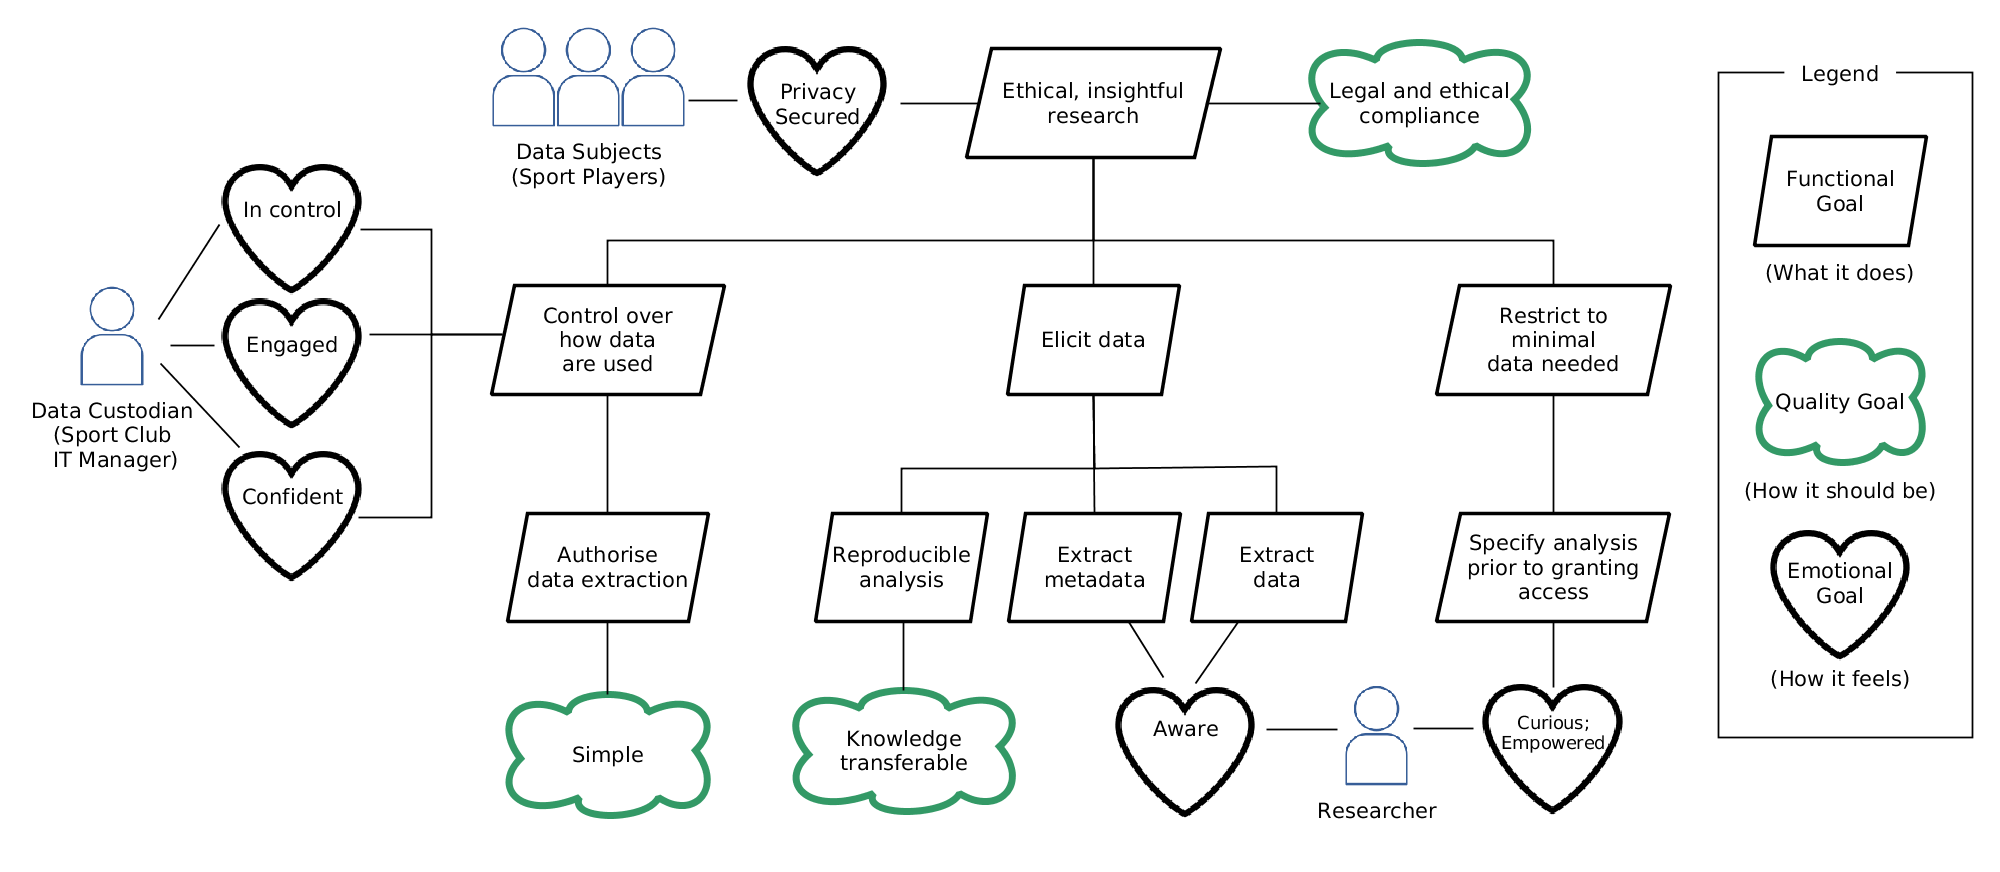
\includegraphics[width=\linewidth]{ozchi-emotional-goals-v7}
  \caption{De-identification portal Emotional Goal Model (diagram should be read top to bottom)}
  \label{fig:deident-emotional-goals}
\end{figure}
\end{landscape}

The overall goal of the de-identification portal is to provide a
platform for ethical, insightful research that facilitates reuse of data
without compromising the privacy of the data subjects (i.e. the sport
players). To achieve this goal, the control over how the data are used
must lie with the data custodian (i.e. the sport club) rather than the
researcher, as providing the researcher with unrestricted access to the
system would be equivalent to transfer of identifiable data without
participant consent. On the other hand, to encourage insightful
research, the system should promote a mindset of intellectual
\emph{curiosity} whereby the researcher feels \emph{empowered} to
request (but not necessarily be granted access to) data and propose
analyses that fully utilise the detail available in the dataset to gain
an \emph{awareness} that is not limited to traditional predefined
summary statistics. To meet the goals of all stakeholders, \figref{fig:deident-emotional-goals} proposes that the researcher should precisely specify the data they need for an analysis by writing a script to perform the extraction. In cases where
an analysis requires access to sensitive data, the extraction script
should perform the analysis on the sensitive data then de-identify the
output to ensure that it is non-identifiable. The data custodian (i.e.
the sport club IT manger) should feel \emph{engaged} in the research
process and \emph{in control} over authorising the execution of a script
so that they can be \emph{confident} the research is protecting the data
subjects' (i.e. the players in their club) right to feel that their
\emph{privacy is secured}.

\subsubsection{Interaction model}\label{sec:deidentify-interactionmodel}

\begin{figure}[htp]
  \centering
  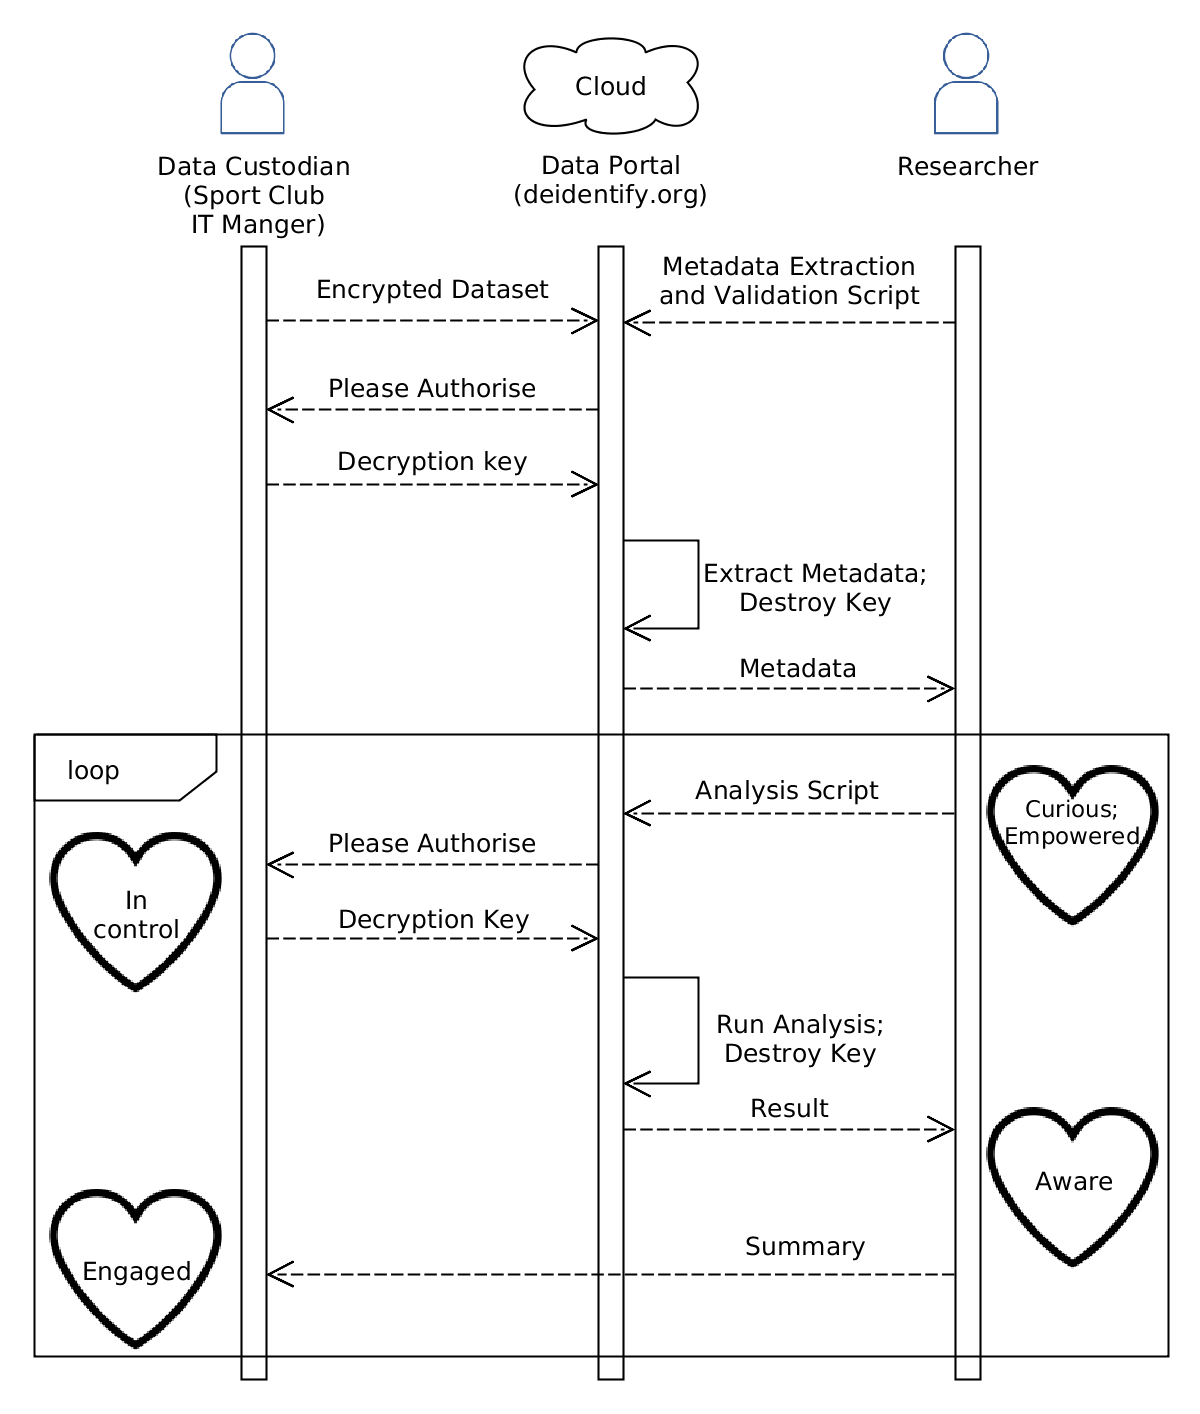
\includegraphics[width=\linewidth]{ozchi-swimlanes_v4}
  \caption{De-identification portal Interaction Model}
  \label{fig:deident-swimlanes}
\end{figure}

\figref{fig:deident-swimlanes} shows the interaction model for the proposed system, and translates the goals into role interactions. This level introduces
the role of a cloud data portal, an autonomous agent that will mediate
the interactions between the data custodian and researcher in a secure
manner. To ensure the data custodian remains in control of data access,
in our solution they encrypt the data prior to uploading the data to the
cloud. The researcher proposes an analysis by uploading a script to the
cloud portal and providing a human readable summary for the data
custodian. If the data custodian is satisfied that the proposed analysis
is respectful of the privacy and rights of the participants, they
authorise the cloud portal to perform the analysis proposed by the
researcher by providing it with the decryption key. The cloud portal
uses the key to temporarily decrypt the data, runs the analysis script
against the raw data, and finally destroys the key after script
execution is complete. Upon completion the researcher is notified so
that they can perform post-analysis on the results of the extraction
script and communicate the results back to the data custodian. This is
an iterative process; the first iteration is usually to extract metadata
and validate the researcher's assumptions about the dataset. The
following iterations deal with extracting data to answer a specific
research question, which may prompt subsequent questions.

As the data custodian is \emph{in control} of the authorisation of each
phase, this has the additional benefit of keeping them emotionally
\emph{engaged} in the research process. As the analysis is run in the
cloud, the researcher never sees the raw data nor the decryption key,
and thus never has access to re-identifiable data; the researcher is
\emph{aware} only of the final output of their analysis, thus
\emph{empowering} the researcher to satisfy their feeling of
\emph{curiosity} about well-formed questions without revealing details
that would compromise the data subjects' privacy.

\subsection{Implementation}

A proof of concept de-identification portal was implemented based on the
above design. A cloud virtual machine was used to host the data portal,
an AES 256-encrypted zip file to protect the dataset, Python script
files for the researcher to express the proposed analysis, an HTML web
interface for the data custodian to authorise a script by providing the
decryption key, and a background process to run the analysis in the
cloud and store the result.

% Generated by https://www.tablesgenerator.com/
% (Locations of breaks manually modified to match paper)
% https://tex.stackexchange.com/questions/50352/inserting-a-small-vertical-space-in-a-table
\begin{landscape}
\begin{table}[]
  \caption{Heuristic Evaluation against ISO Usability Characteristics}
  \footnotesize % https://en.wikibooks.org/wiki/LaTeX/Fonts#Sizing_text
  \label{tab:usability-heuristic}
\begin{tabular}[t]{lllll}
\hline
\begin{tabular}[c]{@{}l@{}}\textbf{ISO Usability}\\   \textbf{Characteristic}\end{tabular} & \textbf{ISO Definition}                                                                                                                                                                                                                                                             & \textbf{Spreadsheet}                                                                                                                                                                                                                                      & \textbf{Ours}                                                                                                                                                                           \\
\hline
\noalign{\vskip 2mm}
\begin{tabular}[t]{@{}l@{}}Appropriateness\\ recognizability\end{tabular}         & \begin{tabular}[t]{@{}l@{}}Degree to which users can recognise\\ whether a product or system is\\ appropriate for their needs.\end{tabular}                                                                                                                                                  & \begin{tabular}[t]{@{}l@{}}Spreadsheet editors are an obvious\\ choice for data custodian to use to\\ remove/substitute participant identifier\\ columns, but data custodian may not\\ be aware of need to also remove quasi-\\ identifiers.\end{tabular} & \begin{tabular}[t]{@{}l@{}}Researcher determines\\ appropriate de-identification\\ methods and sends link and\\ instructions to data custodian.\end{tabular}                            \\
\noalign{\vskip 2mm}
Learnability                                                                      & \begin{tabular}[t]{@{}l@{}}Degree to which a product or system can\\ be used by specified users to achieve\\ specified goals of learning to use the\\ product or system with effectiveness,\\ efficiency, freedom from risk and\\ satisfaction in a specified context of use.\end{tabular}   & \begin{tabular}[t]{@{}l@{}}Spreadsheets provide a familiar and\\ intuitive interface. However, without\\ proper training, there is a risk of data\\ errors due to incorrect formulas that\\ refer to the wrong cells.\end{tabular}                        & \begin{tabular}[t]{@{}l@{}}Researcher must have\\ sufficient training to express\\ de-identification operations.\end{tabular}                                                           \\
\noalign{\vskip 2mm}
Operability                                                                       & \begin{tabular}[t]{@{}l@{}}Degree to which a product or system has\\ attributes that make it easy to operate\\ and control.\end{tabular}                                                                                                                                                     & \begin{tabular}[t]{@{}l@{}}Spreadsheets provide an intuitive\\ interface. However, may be slow and\\ repetitive if need to manually apply the\\ same operation to many worksheets.\end{tabular}                                                           & \begin{tabular}[t]{@{}l@{}}The data custodian only needs\\ to provide encryption/\\ decryption password.\end{tabular}                                                                   \\
\noalign{\vskip 2mm}
\begin{tabular}[t]{@{}l@{}}User error\\ protection\end{tabular}                   & \begin{tabular}[t]{@{}l@{}}Degree to which a system protects users\\ against making errors.\end{tabular}                                                                                                                                                                                     & \begin{tabular}[t]{@{}l@{}}Spreadsheet software has no intrinsic\\ functionality for recognising\\ identifiable data. Responsibility falls on\\ data custodian.\end{tabular}                                                                              & \begin{tabular}[t]{@{}l@{}}Researcher can test their code\\ on a sample data set. Data\\ custodian's role is reduced to\\ choosing an appropriate\\ encryption password.\end{tabular}   \\
\noalign{\vskip 2mm}
\begin{tabular}[t]{@{}l@{}}User interface\\ aesthetics\end{tabular}               & \begin{tabular}[t]{@{}l@{}}Degree to which a user interface enables\\ pleasing and satisfying interaction for\\ the user.\end{tabular}                                                                                                                                                       & \begin{tabular}[t]{@{}l@{}}Spreadsheet provides a familiar and\\ intuitive interface.\end{tabular}                                                                                                                                                        & Interface can be themed.                                                                                                                                                                \\
\noalign{\vskip 2mm}
Accessibility                                                                     & \begin{tabular}[t]{@{}l@{}}Degree to which a product or system can\\ be used by people with the widest range\\ of characteristics and capabilities to\\ achieve a specified goal in a specified\\ context of use.\end{tabular}                                                               & \begin{tabular}[t]{@{}l@{}}Spreadsheets in default mode present\\ issues for users with low vision.\end{tabular}                                                                                                                                          & \begin{tabular}[t]{@{}l@{}}Interface conforms to W3C\\ Web Content Accessibility\\ Guidelines.\end{tabular}                                                                             \\
\hline
\end{tabular}
\end{table}

\end{landscape}

\subsection{Heuristic usability evaluation}

Table~\ref{tab:usability-heuristic} shows results of a heuristic evaluation of our system according to
the usability characteristics defined in the ISO software quality
framework \cite{ISO2011}. In contrast to prescriptive usability heuristic
checklists such as those presented by Nielsen \cite{Nielsen1990}, the focus of this section is on
evaluating usability concerns stemming from the software architecture
\cite{Folmer2004} rather than on minor usability issues that are implementation
specific.

\subsection{Case study} \label{sec:deident-casestudy}

This section shares preliminary experience using the system to
obtain de-identified player position tracking data from a sport club for
team strategy analysis.

To deal with the unique privacy issues associated with human trajectory
data, a custom de-identification operation was selected that combined
downsampling the position data to 1 Hz with a randomly sorted
point~cloud representation to increase uncertainty of player identities
whenever two player paths crossed each other \cite{Ding2017}. As the custom
de-identification operation was too involved for the sport club to
perform themselves, the sport club was asked to encrypt and upload the raw\footnote{The sport club took basic steps to strip out identifying information prior to uploading the data, such as replacing player names with anonymous identifiers, but this in itself would have been insufficient to prevent re-identification attacks.} player position tracking data to the de-identification portal (\textit{deidentify.org}) designed and implemented as part of this thesis.

Implementing the analysis script to extract and de-identify data proved
to be challenging without having a way to peek at the structure of the
underlying raw data it was operating on. While theoretically this could
be addressed through metadata or sample data, in this situation metadata
was not available and the format of the sample data differed from the
actual data. Thus, multiple iterations were necessary to infer the data
structure and to address parsing related issues.

While ultimately successful, the overall process took one month as each
iteration had to wait for manual authorisation by the sport club who
acted as the data custodian.

\subsection{Conclusions}

Our tool and method are simpler for the data custodian at some
additional burden to the researcher when compared against using
a spreadsheet tool such as
Microsoft Excel, the most commonly used tool for this operation
currently. Specifically, our approach calls for the researcher to be
able to express de-identification via an automated script. This
is a superior approach as the researcher would typically have additional
skills and training to handle data compared to the data custodian.

While the case study examined sport club data, the approach is, in
principle, generalisable to other domains in which the data custodian
lacks the technical resources to de-identify the data themselves. Future
work is needed to validate the emotional goal model through interviews
with stakeholders, and to run an empirical trial to quantify the extent
to which the system satisfies the emotional goals of the data custodian
and researcher.

Future implementations could benefit from functionality to automatically
reverse-engineer the structure and semantics of a dataset without
revealing individuals in the dataset; this would reduce the number of
iterations required for the researcher to understand the dataset and
arrive at the final analysis, thus reducing risk of feelings of
irritation and frustration from the data custodian and researcher.

\newpage{}
